% helper macros

\chapter{Introduction}\label{chap1}

%\addtocontents{toc}{\protect\bigskip\centerline{\underline{\textbf{Module  - I}}}} 
\addtocontents{toc}{\protect\contentsline{chapter}{\protect Chapter \numberline{\thechapter.}
  Introduction}{\thepage--\pageref{1end}}}  

\section{Definitions of a Signal}\label{sec1.1}

A signal can be defined as a function that conveys {\em information}. Although signals can be represented in many ways, in all cases the information is contained in some pattern of variations. Signals are represented mathematically as a function of one or more independent variables. If the function depends on a single variable, the signal is said to be {\em one dimensional}. Eg., Speech signal. A speech signal is represented mathematically as a function of time wherein the amplitude varies with time depending on the spoken word and the person who speaks it. If the function depends on two or more variables, the signal is said to be {\em multidimensional}. Eg., Image signal. A photographic image is represented as a brightness function of two special variables.

Usually the independent variable of the mathematical representation of a signal is taken as {\em time}. But in some specific cases the independent variable may not be time.

\noindent
{\bf Real-Life examples for signals}
\smallskip

In this section, we have discussed few examples for real-life signals.
\begin{itemize}
\item[(a)] By listening to the heart-beat of a patient, a doctor is able to diagnose the presence or absence of disease. The quantity (heart-beat) represents signal that convey information to the doctor about the state of health of the patient.

\item[(b)] In listening to a weather forecast over the radio, we get quantities regarding variations in temperature, humidity, the speed of wind etc. The signals represented by these quantities help us to decide whether to go out for a walk or not.
\end{itemize}

Basically there are two types of signals. (i) Continuous-time signal and (ii) Discrete-time signal.

\medskip
\noindent
{\bf (i) Continuous-time signal}
\smallskip

A signal $x(\rmt)$ is said to be a {\em continuous-time signal} if it has value of amplitude for all time `t' (i.e., the independent variable `t' is continuous). Fig. \ref{chap1-fgig1.1} represents an example of a continuous-time signal whose amplitude varies continuously with time. Continuous-time signals arise naturally when a physical phenomenon (eg., heart-beta, acoustic pressure variation etc.) is converted into an electrical signal using appropriate transducer.
\begin{figure}[H]
\centering
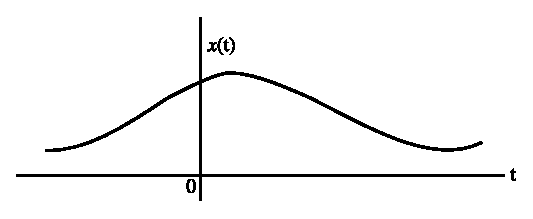
\includegraphics{src/chap1/fig1.eps}
\caption{A continuos time signal}\label{chap1-fig1.1}
\end{figure}

\medskip
\noindent
{\bf (ii) Discrete-time signal}
\smallskip

A discrete-time signal is defined only at discrete instants of time. (i.e. the independent variable has discrete values only which are usually uniformly spaced)

A discrete-time signals are represented mathematically as sequence of numbers. A sequence of numbers $x$ in which the $\rmn^{\text{th}}$ number in the sequence is denoted by $x(\rmn)$ is written as,
$$
x=\{x(\rmn)\}\quad ;~ -\infty<\rmn<\infty
$$
where `$\rmn$' is an {\em integer}.

Practically, such sequences are usually obtained from a continuous - time signal by sampling it at a uniform rate.

Consider `$\tau$' is the sampling period and `$n$' denote an integer $(-\infty<\rmn<\infty)$. Sampling a continuous-time signal $x(\rmt)$ at time $\rmt=\rmn\tau$ gives a sample value $x(\rmn\tau)$. We write this sampled signal as $x(\rmn)$ such that,
$$
x(\rmn)=x(\rmn\tau)\quad ;~ \rmn=0, \ \pm 1, \ \pm 2, \ \pm 3,\ldots
$$

Thus a discrete-time signal is represented by a sequence numbers $\ldots x(-2)$, $x(-1)$, $x(0)$, $x(1)$, $x(2)\ldots$.

Fig. \ref{chap1-fig1.2}(a) and (b) illustrates the relationship between a continuous-time signal $x(\rmt)$ and discrete-time signal $x(\rmn)$ derived from it.
\begin{figure}[H]
\centering
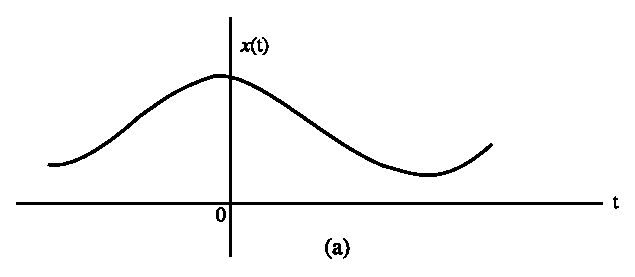
\includegraphics{src/chap1/fig2.eps}
\end{figure}
\bigskip

\begin{figure}[H]
\centering
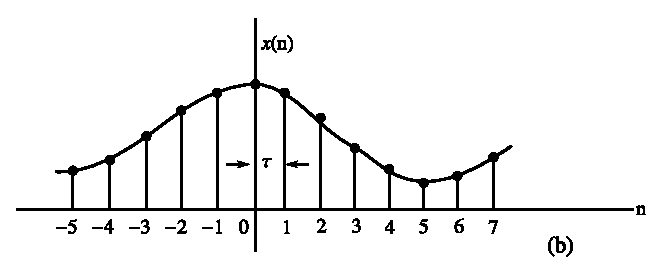
\includegraphics{src/chap1/fig3.eps}
\caption{Discrete time signal $x(\rmn)$ obtained from a continuous-time signal $x(\rmt)$ with sampling perior `t'}\label{chap1-fig1.2}
\end{figure}

\section{Definitions of a System}

A {\em system} is an interacting group of physical objects or physical conditions that are called system {\em components}. A physical system is an interconnection of components, devices or subsystems.

Signals that enter a system from some external source are referred to as {\em input signals}. Signals produced by the system by processing the input signals are called the {\em output signals} or {\em responses}. Signals that occur within a system and therefore are neither input nor output signals are called {\em internal signals}. The system responds to one or more input signals to produce one or more output signals. These signals are functions of an independent variable such as time, distance etc.

Many systems are quite complex. They may contain system components and signals of different types. For example, an audio amplifier system contains microphone that convert acoustic signals to electrical signals, amplifier that amplify the electrical signals and speakers that convert electrical signals to acoustic signals.

A {\em continuous time system} is one where continuous time input signals are applied which results in continuous time output signals. It can be represented pictorially as shown in Fig. \ref{chap1-fig1.3}.
\begin{figure}[H]
\centering
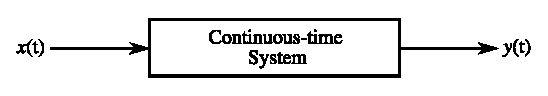
\includegraphics{src/chap1/fig4.eps}
\caption{A representation for continuous-time system}\label{chap1-fig1.3}
\end{figure}
where $x(\rmt)$ is the input signal and $y(\rmt)$ is the output signal.

Alternatively, we can represent the input-output relation of a continuous time system by the notation as written below.
$$
x(\rmt)\to y(\rmt)
$$

Similarly, a {\em discrete-time system} is one where discrete-time input signals are applied which results in discrete-time output signals. It can be represented pictorially as shown in Fig. \ref{chap1-fig1.4}.
\begin{figure}[H]
\centering
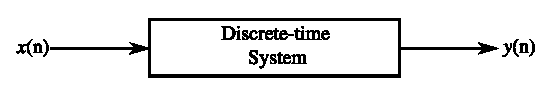
\includegraphics{src/chap1/fig5.eps}
\caption{A representation for discrete-time system}\label{chap1-fig1.4}
\end{figure}
where $x(\rmn)$ is the input signal and $y(\rmn)$ is the output signal.

Alternatively, we can represent the input and output relation of a discrete-time system by the notation as written below.
$$
x(\rmn)\to y(\rmn)
$$

Examples for systems
\begin{figure}[H]
\centering
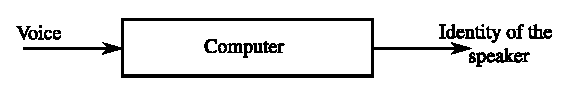
\includegraphics{src/chap1/fig6.eps}
\caption{Automatic speaker recognition system}\label{chap1-fig1.5}
\end{figure}
\begin{figure}[H]
\centering
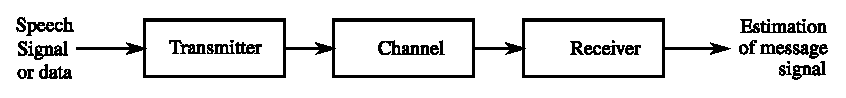
\includegraphics{src/chap1/fig7.eps}
\caption{Communication system}\label{chap1-fig1.6}
\end{figure}

\medskip
\noindent
{\bf Real-Life Examples for Systems}
\smallskip

In this section, we will discuss some of the real-life systems in brief.

\bigskip
\noindent
{\it\bfseries 1. Communication Systems :}
\smallskip

The three basic elements of communication system are (i) Transmitter (ii) Channel (iii) Receiver as shown in Fig. \ref{chap1-fig1.6}. The {\em transmitter} and {\em receiver} are places at a distance apart which are connected by a physical medium called {\em channel}. The channel may be free space, optical fiber, co-axial cable etc. The transmitter converts the message signal (eg., speech signal, video signal etc.) produced by a source of information into a form suitable for transmission over the channel. When the transmitted signal travels through the channel it would be distorted due to the physical characteristics of the channel. In addition to this, noise and interfering signals originating from other sources contaminate the message signals. The receiver receives the distorted signal to reconstruct it into a recognizable form or into an estimated form of the original message signal.

Thus, the receiver does the reverse process that of transmitter and also reverses the effect of the channel such as noise elimination, amplification of weak signals etc.

\bigskip
\noindent
{\it\bfseries 2. Control Systems :}
\smallskip

Fig. \ref{chap1-fig1.7} shows the block diagram representation of a closed-loop control system or feedback control system.
\begin{figure}[H]
\centering
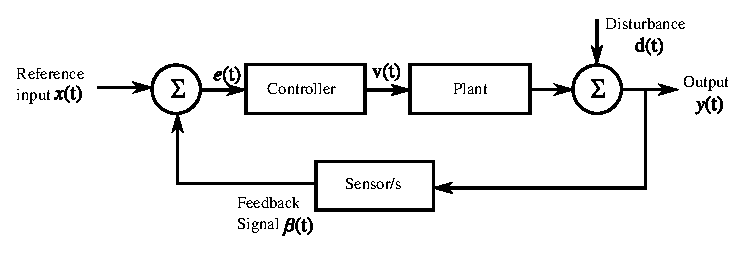
\includegraphics{src/chap1/fig8.eps}
\caption{Block diagram of closed loop control system}\label{chap1-fig1.7}
\end{figure}

In any control system, the plant is represented by mathematical operations that generate the output $y(\rmt)$ in response to the plant input $v(\rmt)$ and the external disturbance $d(\rmt)$. The sensors existing in the feedback loop measures the plant output $y(\rmt)$ and converts it into another form $\beta(\rmt)$ known as {\em feedback signal}. It is compared against the reference input $x(\rmt)$ to produce an {\em error signal} $e(\rmt)$. This error signal is applied to a controller which in turn produces the {\em actuating signal} $v(\rmt)$ that performs the controlling action of the plant.

For example, in an aircraft landing system, the plant is represented by the aircraft body and actuator. The sensors are used by the pilot to determine the lateral position of the aircraft and the controller is a digital computer.

\bigskip
\noindent
{\it\bfseries 3. Remote Sensing Systems :}
\smallskip

Remote sensing is defined as the process of acquiring informations about and object of interest without being in physical contact with it. The acquisition of informations is accomplished by detecting and measuring the changes that the object creates on the surrounding field. This field may be electromagnetic, acoustic, magnetic etc.

The acquisition of informations can be done in a passive manner by listening to the field that is naturally emitted by the object and processing it or by purposely illuminating the object with a defined field and processing the echo.

\section{Elementary Continuous-Time Signals}\label{chap1-sec1.3}

The {\em elementary} of {\em basic} signals occur frequently in nature. These signals are the basic building blocks for constructing more complex signals. Many physical signals that occur in nature can be modelled using these elementary signals.

Some of the important elementary continuous-time signals are,
\begin{itemize}
\item[(i)] Exponential signals

\item[(ii)] Sinusoidal signals

\item[(iii)] Exponentially damped sinusoidal signals

\item[(iv)] Unit step function

\item[(v)] Unit impulse function

\item[(vi)] Unit ramp function
\end{itemize}

\subsection{Exponential Signals}\label{chap1-sec1.3.1}

A real exponential continuous-time signal is given by
\begin{equation}
x(\rmt)=\rmC\; \rme^{\at}\label{chap1-eq1.1}
\end{equation}
where both `$\rmC$' and `$\rma$' real constant. In Eqn. \eqref{chap1-eq1.1}, `$\rmC$' is known as the {\em amplitude} of the exponential signal at $\rmt=0$.

If $\rma<0$ (i.e., `$\rma$' is negative), the signal $x(\rmt)$ is known as {\em decaying exponential signal} and if $\rma>0$ (i.e., `$\rma$ is positive) then $x(\rmt)$ is called {\em growing exponential signal}.

Fig. \ref{chap1-fig1.8}(a) and (b) shows the real decaying and growing exponential signal respectively.

\begin{figure*}[t!]
\centering

\begin{subfigure}[t]{0.4\textwidth}
\centering
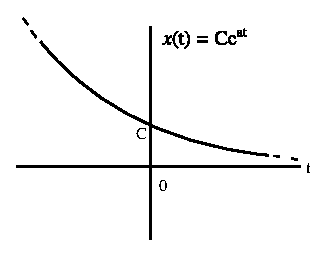
\includegraphics{src/chap1/fig9a.eps}
\caption{Real decaying exponential signal (i.e., $\rma<0$)}\label{chap1-fig1.8a}
\end{subfigure}
\qquad
\begin{subfigure}[t]{0.4\textwidth}
\centering
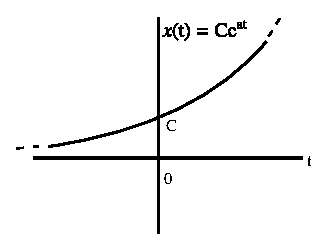
\includegraphics{src/chap1/fig9b.eps}
\caption{Real growing exponential signal (i.e., $\rma>0$}\label{chap1-fig1.8b}
\end{subfigure}
\caption{}\label{chap1-fig1.8}
\end{figure*}


In Eqn. \eqref{chap1-eq1.1}, if `$\rmC$' or `$\rma$' or both are complex numbers, then $x(\rmt)$ is known as {\em continuous-time complex exponential signal}.

\medskip
\noindent
{\it\bfseries Note~:} In Eqn.~\eqref{chap1-eq1.1}, consider $\rmC=1$ and `$\rma$' is imaginary.
\begin{equation}
\text{i.e.,}\quad x(\rmt)=e^{j\omega_{o}\rmt}\label{chap1-eq1.2}
\end{equation}

The signal $x(\rmt)$ given by Eqn. \eqref{chap1-eq1.2} is periodic with fundamental period $\rmT=\dfrac{2\pi}{\omega_{o}}$. A continuous-time signal $x(\rmt)$ is periodic with period $\rmT$,
\begin{align}
\text{if}\quad x(\rmt) &= x(\rmt+T)\notag\\
x(\rmt) &= e^{j\omega_{o}\rmt}\label{chap1-eq1.3}\\
\therefore\quad x(\rmt+\rmT) &= e^{j\omega_{o}(\rmt+\rmT)}\label{chap1-eq1.4}
\end{align}

for $x(\rmt)$ to be periodic
\begin{align}
e^{j\omega_{o}\rmt} &= e^{j\omega_{o}(\rmt+\rmT)}\notag\\
e^{j\omega_{o}\rmt} &= e^{j\omega_{o}\rmt}\cdot e^{j\omega_{o}\rmT}\label{chap1-eq1.5}
\end{align}

Eqn. \eqref{chap1-eq1.5} is valid only if
\begin{gather}
e^{j\omega_{o}\rmT}=1\notag\\
\therefore\quad \text{If~~ } \omega_{o}=0\quad\text{then}\quad e^{j\omega_{o}\rmT}=1\label{chap1-eq1.6}
\end{gather}

If $\omega_{o}\neq 0$, then the fundamental period $\rmT$ of $x(\rmt)$ is the smallest value of $\rmT$ and is given by,
\begin{equation}
\rmT=\dfrac{2\pi}{\omega_{o}}\label{chap1-eq1.7}
\end{equation}

Substituting Eqn. \eqref{chap1-eq1.7} in Eqn. \eqref{chap1-eq1.6} we get,
\begin{equation}
e^{j\omega_{o}\frac{2\pi}{\omega_{o}}}=e^{j2\pi}=\cos 2\pi + \rmj\sin 2\pi =1\label{chap1-eq1.8}
\end{equation}

Therefore $e^{\rmj\omega_{o}\rmt}$ and $e^{-\rmj\omega_{o}\rmt}$ are periodic with fundamental period $T=\dfrac{2\pi}{\omega_{o}}$.

\subsection{Sinusoidal signals}\label{chap1-eq1.3.2}

A sinusoidal signal is given by,
\begin{equation}
x(\rmt)=A\cos (\omega_{o}\rmt+\phi)\label{chap1-eq1.9}
\end{equation}
where
\begin{align*}
\omega_{o}=2\pi \rmf_{o} &= \text{angular frequency (rad/sec)}\\
\rmf_{o} &= \text{linear frequency~  (Hz)}\\
\phi &= \text{phase shift\quad (radians)}
\end{align*}
The fundamental period of the signal $x(\rmt)$ in Eqn. \eqref{chap1-eq1.9} is $\rmT=\dfrac{2\pi}{\omega_{o}}$ (sec.)

\subsection{Exponential damped sinusoidal signals}\label{chap1-sec1.3.3}

An exponentially damped sinusoidal signal is given by,
$$
x(\rmt)=e^{-\at}\sin \omega \rmt\quad ;~ \text{where~ } \rma >0
$$
As `$\rmt$' increases, the amplitude of sinusoidal oscillation decreases exponentially and approaches zero as $\rmt\to \infty$. An exponentially damped sinusoidal signal is shown in Fig. \ref{chap1-fig1.9}.
\begin{figure}[H]
\centering
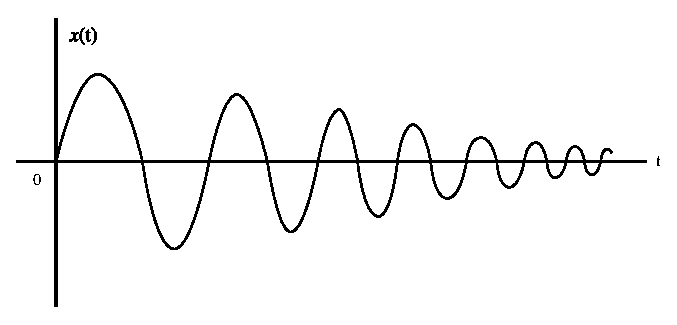
\includegraphics{src/chap1/fig10.eps}
\caption{An exponentially damped sinusoidal signal}\label{chap1-fig1.10}
\end{figure}

\subsection{Unit step function : $\rmu(\rmt)$}\label{chap1-sec1.3.4}

The continuous-time unit step function is defined as,
\begin{align*}
\rmu(\rmt) &= 1\quad ;~ \rmt\geq 0\\
     &= 0\quad ;~ \rmt<0
\end{align*}

It is shown in Fig. \ref{chap1-fig1.10}
\begin{center}
{\bf Figure 1.10}
\end{center}

\subsection{Unit impulse function : $\delta(\rmt)$}\label{chap1-sec1.3.5}

The continuous-time unit impulse function $\delta(\rmt)$ is defined as,
\begin{align}
\delta(\rmt) &= 0\quad ;~ \rmt\neq 0\notag\\
\text{and}\quad \int\limits^{\infty}_{-\infty}\delta(\rmt)\dt &=1\label{chap1-eq1.10}
\end{align}

This function $\delta(\rmt)$ is also known as {\em Dirac delta function}.

The continuous-time unit impulse function $\delta(\rmt)$ is shown in Fig. \ref{chap1-fig1.11}
\begin{center}
{\bf Figure 1.11}
\end{center}

Eqn. \eqref{chap1-eq1.10} indicates that the area covered by an unit impulse function is {\em unity}.

The impulse function $\delta(\rmt)$ is the derivative of the step function with respect to time.

Consider a non-idealized unit step function $u_{\Delta}(\rmt)$ as shown in Fig. \ref{chap1-fig1.12}(a). The derivative of $\rmu_{\Delta}(\rmt)$ with respect to time `$t$' is shown in Fig. \ref{chap1-fig1.12}(b).
\begin{center}
{\bf Figure 1.12(a) and (b)}
\end{center}
\begin{equation}
\delta_{\Delta}(\rmt)=\dfrac{\du_{\Delta}}{\dt}(\rmt)\label{chap1-eq1.11}
\end{equation}

The area of function $\delta_{\Delta}(\rmt)=\Delta \cdot \dfrac{1}{\Delta}=1$. In Fig. \ref{chap1-fig1.12}(b), as $\Delta\to 0$,

$\delta_{\Delta}(\rmt)$ becomes narrower and higher maintaining its unit area.
\begin{equation}
\delta(\rmt)=\Lt\limits_{\Delta \to 0}\delta_{\Delta}(\rmt)\label{chap1-eq1.12}
\end{equation}

Therefore unit impulse function has,
\begin{itemize}
\item[(i)] Zero width

\item[(ii)] Infinite height

\item[(iii)] Unit area or unit strength
\end{itemize}

A graphical representation of impulse function with strength `$\rmk$' is shown in Fig. \ref{chap1-fig1.13}. The strength `$\rmk$' indicates the area under the impulse.
\begin{center}
{\bf Figure 1.13}
\end{center}

\medskip
\noindent
{\bf Properties of continuous-time Impulse function :}
\begin{itemize}
\item[(i)] $\int\limits^{\infty}_{-\infty}\delta(\rmt)\dt=1$

\item[(ii)] $\int\limits^{\infty}_{-\infty}\rmk \ \delta (\rmt)=k$

\item[(iii)] $x(\rmt)\delta(\rmt)=x(0)\delta(\rmt)$

\item[(iv)] $\int\limits^{\infty}_{-\infty}x(\rmt)\delta(\rmt)\dt=x(0)$

\item[(v)] $x(\rmt)\cdot \delta(\rmt-\rmt_{o})=x(\rmt_{o})\delta(\rmt-\rmt_{o}) \ \Rightarrow$ (sampling property of impulse function)

\item[(vi)] $\int\limits^{\infty}_{-\infty}x(\rmt)\delta(\rmt-\rmt_{o})\dt=x(\rmt_{o}) \ \Rightarrow$ (sifting property of impulse function)

\item[(vii)] $\delta(\at)=\dfrac{1}{\rma}\delta(\rmt)$\quad ;~$\rma>0$
\end{itemize}

\subsection{Unit ramp function $r(\rmt)$}

\begin{tabbing}
A ramp function is defined as $\rmr(t)$ \== t\quad~;~ t $\geq 0$\\
                                        \>= 0\!\quad~;~ t $<0$
\end{tabbing}

It is the integral of the unit step function $\rmu(\rmt)$. An unit ramp function is shown in Fig.~\ref{chap1-fig1.14}.
\begin{figure}[H]
\centering
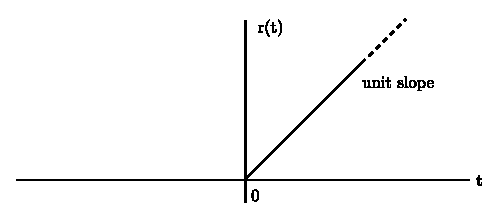
\includegraphics{src/chap1/fig.1.14.eps}
\caption{An unit ramp function}\label{chap1-fig-1.14}
\end{figure}

\section{Elementary Discrete-Time Signals}\label{chap1-sec1.4}
The elementary discrete-time signals are direct counterparts of the continuous-time signals described in section
\ref{chap1-sec1.3}. Many of the characteristics of basic discrete-time signals are directly analogous to that of basic continuous-time signal form that of continuous-time signal. 

Some of the important basic discrete-time signal are,
\begin{itemize}
\item[(i)] Exponential signals.

\item[(ii)] Sinusodial signals.
 
\item[(iii)] Exponentially damped sinusoidal signals.

\item[(iv)] Unit step sequence.
 
\item[(v)] Unit impulse sequence.

\item[(iv)] Unit ramp sequence. 
\end{itemize}

\subsection{Discrete-time Exponential Signals}\label{chap1-subsec-1.4.1}
A real exponential discrete-time signal or sequence is given by,
\begin{align}
x(n) &= \rmC \alpha^{n}\label{chap1-eq-1.13}\\
\text{where}\qquad \alpha &= e^{\beta}\label{chap1-eq-1.14}
\end{align}

and C, $\alpha$ and $\beta$ are real constants. In eqn.\ref{chap1-eq-1.13} `C' is known at the \textit{amplitude} of the sequence at $n=0$. If $|\alpha| < 1$, the signal decays exponentially. Furthermore, if $\alpha < 0$ (i.e, $\alpha$ is negative), then the sign of $x(n)$ alternates i.e, when `n' is positive, $x(n)$ has positive value and when `n' is negative, $x(n)$ has negative value.

The plos of $x(n) = \rmC \alpha^{n}$ for $\alpha > 1; 0< \alpha < 1 ; -1 < \alpha < 0$ and $\alpha < -1$  are shown in Fig. \ref{chap1-fig-1.29} (a), (b), (c) and (d) respectively.

In eqn. \ref{chap1-eq-1.13}, if $`\rmC'$ or $`\alpha'$ or both are complex numbers, then $x(n)$ is known as \textit{discrete-time complex exponential sequence},

\begin{center}
{\bf 1.4.1 fig-1.15  (4 figures add)}
\end{center}

\noindent
\textit{Note~:} In eqn. \ref{chap1-eq-1.13} and eqn.\ref{chap1-eq-1.14}. Consider $\rmC=1$ and and $\beta$ is purely imaginary.
\begin{equation}
\text{i.e.}, \qquad  x(n)= e^{j\Omega_{o}n}\label{chap1-eq-1.15}
\end{equation} 

The complex exponential discrete-time signal $x(n)= e^{j\Omega_{o}n}$  is periodic with fundamental period $N$ if,
\begin{equation}
\dfrac{\Omega_{o}}{2 \pi} = \dfrac{m}{N}\label{chap1-eq-1.16}
\end{equation}

where $`m'$  is an integer (i.e, $\frac{\Omega_{o}}{2\pi}$ must be a rational number)

A discrete-time signal $x(n)$ is periodic with period $N$, if
\begin{align}
x(n) &= x(n + N)\notag\\
x(n) &= e^{j \Omega_{o}n}\notag\\
\therefore x(n + N)&= e^{j \Omega_{o}(n + N)}\label{chap1-eq-1.17}\\ 
\therefore x(n + N)&= e^{j \Omega_{o}n} \cdot e^{j \Omega_{o} N}=x(n)= e^{j \Omega_{o}n} \quad \text{if and only if},\notag\\
e^{j \Omega_{o} N} &= 1\label{chap1-eq-1.18}
\end{align}
\begin{equation}
\text{Eqn. \ref{chap1-eq-1.18} is satisfied  only if either} \quad \Omega_{o} = 0\quad \text{or} \quad
\Omega_{o}N= 2\pi m\label{chap1-eq-1.19}
\end{equation}
where $`m'$ is an integer.
\begin{equation}
\therefore \dfrac{\Omega_{o}}{2 \pi}  = \dfrac{m}{N}\label{chap1-eq-1.20}
\end{equation}
Therefore discrete-time complex exponential signal is periodic only if $\Omega_{o}$ is a rational multiple of $2\pi$.
\begin{equation}
\text{i.e.},  \quad \Omega_{o} = 2\pi \cdot \dfrac{m}{N}\label{chap1-eq-1.21}
\end{equation}

Where `$N$' i fundamental period $\Omega_{o}$ is angular frequency is radians (if `$n$' is  dimensionless) and `$m$' is an integer.

\subsection{Discrete-time Sinusoidal Signals}\label{chap1-subsec-1.4.2}

A discrete-time version of a sinusoidal signal is given by
\begin{equation}
x(n) = \rmA \cos (\Omega_{o}n + \Phi)\label{chap1-eq-1.22}
\end{equation}
where `$A$' is maximum value of $x(n)$, $\Omega_{o}$ is angular frequency and $\Phi$ is phase angle.

If `$n$' is dimensionless,both $\Omega_{o}$ and $\Phi$ are measured in radians.

Unlike continuous-time sinusoidal signal, discrete-time sinusoidal signals are note periodic for an arbitrary values of $\Omega_{o}$. For a discrete-time sinusoidal signal to be periodic, the angular frequency $\Omega_{o}$ must be a rational multiple of $2 \pi$.
\begin{equation}
\text{i.e.}, \qquad \Omega_{o} = 2 \pi\cdot \dfrac{m}{N}\label{chap1-eq-1.23}
\end{equation}
where `$m$' and `$N$' are integers.

Consider a signal $x(n)$ shown in \ref{chap1-Fig-1.16} which is given by,
\begin{equation}
x(n)= \cos\left(\dfrac{\pi n}{4}\right)\label{chap1-eq-1.24}
\end{equation}

Comparing eqn. \ref{chap1-eq-1.24} with eqn. \ref{chap1-eq-1.22}, we have
$$
A = 1, \quad \Phi = 0 \quad \text{and}\quad \Omega_{o} = \dfrac{\pi}{4} = \dfrac{2\pi}{ 8} = 2\pi\cdot \dfrac{1}{8} 
$$

$\therefore$ Fundamental period $N = 8$.
$$
x(n)= \cos \left(\dfrac{\pi n}{4} \right)
$$

\begin{center}
 chap1 fig 1.16 ??????????? add
\end{center}


\subsection{Discrete-time exponentially damped sinusoidal signals}\label{chap1-subsec-1.4.3}

A discrete-time exponentially damped sinusoidal sequence  is given by,
\begin{equation}
x(n) = \rmC \alpha^{n} \sin(\Omega n + \Phi) \quad ; 0 < |\alpha| < 1 \label{chap1-eq-1.25}
\end{equation}

The value of $x(n)$ decreases as `$n$' increases.

\subsection{Discrete-time unit step sequence : $u(n)$}\label{chap1-subsec-1.4.4}

A discrete-time unit step sequence is defined as,
\begin{align*}
u(n) &= 1 \quad ; n \geq 0\\
&= 0\quad ; n < 0
\end{align*}

It is shown in Fig \ref{chap1-fig-1.17}
\begin{center}
chap1-fig 1.17 ???????? add
\end{center}

\subsection{Discrete-time unit impulse sequence : $\delta(n)$}\label{chap1-subsec-1.4.5}

A discrete-time impluse sequence is defined as,
\begin{align*}
\delta(n) &= 1  \quad; n=0\\
& =0 \quad; n \neq 0
\end{align*}

It is shown in Fig. \ref{chap1-fig-1.18}

\begin{center}
chap1 fig 1.18 ??????? add
\end{center}

\noindent
{\it\bfseries Properties if discrete-time Impulse sequence:} 
\begin{center}
\begin{tabular}{ll}
(i)   & $x(n)\delta(n)= x(0)\delta(n)$ \quad\qquad (ii)~~  $x(n)\delta(n_{o})\delta(n-n_{o})$  \\
(iii) & $\sum\limits_{n= -\infty}^{\infty}x(n)\delta(n) = x(0)$\\
(iv) & $\sum\limits_{n=-\infty}x(n)\delta(n-n_{o}) =x(n_{o})$ \quad \text{(sifting property of impulse sequence)}
\end{tabular}
\end{center}

\noindent
{\it \bfseries Note~:}
\begin{align*}
\rmu(\rmn) &= 1 \quad; \rmn \geq 0\\
 &= 0 \quad ; n < 0\\
 \rmu (\rmn) &= \delta(\rmn) + \delta(\rmn-1) + \delta(\rmn-2) + \cdots + \delta(\rmn-\infty)\\
 \rmu (\rmn) &= \sum\limits_{\rmk =0}^{\infty} \delta(\rmn -\rmk)\quad \text{and also} \quad \rmu(\rmn) = \sum\limits_{k=-\infty}^{\rmn} \delta(\rmk) 
\end{align*}

\subsection{Discrete-time unit ramp sequence : $\rmr (\rmn)$}\label{chap1-subsec-1.4.6}

A descrete-timne ramp sequence is defined as,
\begin{align*}
\rmr(\rmn) &= \rmn \quad ; \rmn \geq 0\\
 & = 0 \quad ; \rmn < 0
\end{align*}

It is shown in Fig \ref{chap1-fig-1.19}
\begin{center}
chap1 fig1.19 ??????? add 
\end{center}

\section{BASIC OPERATIONS ON SIGNALS}\label{chap1-sec-1.5}

In this section, we describe some of the basic operations that could be performed on signals. One dimensional signal can be defined using two variables.

(i) Dependent variable \qquad (ii) Independent variable.

Dependent variable corresponds to the amplitude or value of the signal but the independent variable is time `$\rmt$' or
`$\rmn$' for continuous time and discrete-time signal respectively

\subsection{Operations performed on the dependent variables}\label{chap1-subsec-1.5.1}
\begin{itemize}
\item[{\rm a)}]{\it \bfseries Amplitude scaling:} Let $x(\rmt)$ be a continupous time signal. Then the signal
\begin{equation}
y({\rmt}) = {\rmc}  x(\rmt)\label{chap1-eq-1.26}
\end{equation}
is known as amplitude scaled version of $x ({\rmt})$ where `${\rmc}$' is known as \textit{scaling factor}. The signal $\rmy (\rmt)$ is obtained by multiplying the value (amplitude) of $x (\rmt)$  by scalar `$\rmc$' at all `$\rmt$'.

Similarly, let $x (\rmn)$ be a discrete-time signal. Then the signal,
\begin{equation}
{\rmy} ({\rmn}) = {\rmc} x {(\rmn)}\label{chap1-eq-1.27}  
\end{equation}
is known as amplitude scaled version of $x (\rmn)$ where `$\rmc$' is a \textit{scaling factor}. The signal $\rmy(\rmn)$ is obtained by multiplying the value of $x (\rmn)$ by scalar `$\rmc$' at all `$\rmn$'.

\item [{\rm b)}] {\it \bfseries Addition:} Let $x_{1}(\rmt)$ and $x_{2}(\rmt)$ are continuous-time signals. Then the signal,
\begin{equation}
{\rmy}{(\rmt)} = x_{1}{(\rm)} + x_{2}{(\rmt)}\label{chap1-eq-1.28}
\end{equation}
is known as the addition of $x_{1}{(\rmt)}$ and $x_{2}{(\rmt)}$. The value of ${\rmy} {(\rmt)}$ is obtained by adding the values of $x_{1}{(\rmt)}$ and $x_{2}{(\rmt)}$ for all `${\rmt}$'.

Similarly, let $x_{1}{(\rmn)}$ and $x_{2}{\rm(n)}$ are discrete-time signals. Then the signal,
\begin{equation}
{\rmy}{(\rmn)} = x_{1} {(\rmn)} + x_{2}{\rmn}\label{chap1-eq-1.29}
\end{equation}
is known are the addition of $x_{1}{\rm(n)}$ and $x_{2}{\rm(n)}$. The value of ${\rmy}{(\rmn)}$. The value of ${\rmy}{(\rmn)}$ is obtained by adding the values of $x_{1}{(\rmn)}$ for all `${\rmn}$'.

\item[{\rm c)}]{\it \bfseries Multiplication:} Let $x_{1}{(\rmt)}$ and $x_{2}{(\rmt)}$ are given continuous-time signals. Then the signal,
\begin{equation}
{\rmy}{(\rmt)} = x_{1}{(\rmt)} \cdot x_{2}{(\rmt)}\label{chap1-eq-1.30}
\end{equation}
is known as the multiplication of $x_{1}{(\rmt)}$ and $x_{2}{(\rmt)}$. The value or amplitude of $\rmy(\rmt)$ is obtained by taking the product of the values of $x_{2}(\rmt)$ and $x_{2}(\rmt)$ for all `$\rmt$'.

Similarly, let $x_{2}(\rmn)$ and $x_{2}(\rmn)$ are discrete-time signals. Then signal,
\begin{equation}
\rmy(\rm  n) = x_{1}(\rmn), x_{2}(\rmn)\label{chap1-eq-1.31}
\end{equation}
is known as the multiplication of $x_{1}(\rmn)$ and $x_{2}(\rmn)$. The value of $\rmy(\rmn)$ is obtained by taking the production of the values of $x_{1}(\rmn)$ and $x_{2}(\rmn)$ for all `$\rmn$'.

\item[{\rm d)}]{\it \bfseries Differentiation:} Let $x(\rmt)$ be a continuous-time signal. Then the differentiation of $x(\rmt)$  with respect to time `$\rmt$' is defined as,
\begin{equation}
\rmy(\rmt) = \dfrac{{\rmd} x{(\rmt)}}{\rmd \rmt}\label{chap1-eq-1.32}
\end{equation}

\item[{\rm d)}]{\it \bfseries Integrations:} Let $x(\rmt)$ be a continuous-time signal. Than the integration of $x(\rmt)$ with respect to `$\rmt$' is defined as,
\begin{equation}
\rmy(\rmt)= \int\limits_{-\infty}^{\rmt}x(\tau)\rmd \; \tau\label{chap1-eq-1.33}
\end{equation}
\end{itemize}

\subsection{Operations performed on the independent variables}\label{chap1-subsec-1.5.2}

\begin{itemize}
\item[{\rm a)}]{\it \bfseries Time Scaling:} Let $x(\rmt)$ be a continuous-time signal. The signal Man $\rmy(\rmt)$ obtained by scaling the independent variable `$\rmt$' by a factor `$\rma$' is given by,
\begin{equation}
{\rmy}{(\rmt)}= x {(\rma\rmt)}\label{chap1-eq-1.34}
\end{equation}


If ${\rma} > 1$. The signal $\rmy{(\rmt)}$ is compressed version of $x{(\rmt)}$ and if $0 < {\rma} < 1$, the signal $\rmy{(t)}$ is an expanded version of $x{(\rmt)}$.

Eg. Let $x(\rmt)$ is as shown in Fig. \ref{chap1-fig-1.20}

\begin{center}
chap1 fig-1.20 ???????? add
\end{center}

The signal $x(2 \rmt)$ and $x\left(\frac{1}{2}\rmt\right)$ are shown in Fig.\ref{chap1-fig-1.21} respectively.
\begin{center}
chap1 fig-1.21 ???????? add
\end{center}
\begin{center}
chap1 fig-1.22 ???????? add
\end{center}

In the discrete-time sequence.
\begin{equation}
{\rmy}{(\rmn)}= x{(\rmk\rmn)} \quad ; \rmk > 0\label{chap1-eq-1.35}
\end{equation}
where `$\rmk'$ is an integer. If $\rmk>1$, some samples of $x(\rmn)$ would be lost.

Eg. Let $x(\rmn)$ is shown in Fig. \ref{chap-fig-1.23}
\begin{center}
chap1 fig-1.23 ???????? add
\end{center}

The signal $x(2\rmn)$ is shown below in Fig. \ref{chap1-fig-1.24}
\begin{center}
chap1 fig-1.24 ???????? add
\end{center}

\item[{\rm b)}] {\it \bfseries Time Shifting:} Let $x(\rmt)$ be a continuous-time. Then the signal,
\begin{equation}
{\rmy}{(\rmt)} = x{(\rmt-\rmt_{\rmo})}\label{chap1-eq-1.36}
\end{equation}
is known as time shifted version of $x(\rmt)$, where  `$\rmt_{\rmo}$' is the time shift

If $\rmt_{\rmo}>0$ the waveform of the signal is shifted to the right. If $\rmt_{\rmo}< 0$ the waveform is shifted to the left. Let $x(\rmt)$ is shown in Fig. \ref{chap1-fig-1.25}. 
\begin{center}
chap1  fig-1.25 add ????
\end{center}

Then, $x(\rmt-2)$ and $x(\rmt+3)$ is shown in Fig. \ref{chap1-fig-1.26} and \ref{chap1-fig-1.27} respectively.
\begin{center}
chap1  fig-1.26 add ????
\end{center}
\begin{center}
chap1  fig-1.27 add ????
\end{center}

\item[{\rm c)}] {\it \bfseries Reflection:} Let $x(\rmt)$ be a continuous-time signal. Then the signal
${\rmy}{(\rmt)} = x{(-\rmt)}$ is known as the reflected version of $x(\rmt)$ about the amplitude axis.

Example for a continuous-time $x(\rmt)$ and it s reflected version $x(-\rmt)$ is shown in Fig. \ref{chap1-fig-1.28} and \ref{chap1-fig-1.29} respectively.
\begin{center}
chap1  fig-1.28 add ????
\end{center}
\begin{center}
chap1  fig-1.29 add ????
\end{center}

{\bfseries Precedence Rule:} Let the signals $x(\rmt)$ and $\rmy(\rmt)$ are related by the following
eqn. \ref{chap1-eq-1.37}.
\begin{equation}
{\rmy}{(\rmt)}=x {(\rma\rmt-\rmb)}\label{chap1-eq-1.37}
\end{equation}

To get $\rmy(\rmt)$ from $x \rm(\rmt)$, we have to preform both time shifting and time scaling operations.

Put $\rmt=0$ in eqn. \ref{chap1-eq-1.37} we get,
\begin{equation}
{\rmy}(0)=x {(-\rmb)}\label{chap1-eq-1.38}
\end{equation}

Put $\rmt=\rmb/\rma$ in eqn. \ref{chap1-eq-1.37} we get,
\begin{equation}
{\rmy}{(\rmb/\rma)}=x(0)\label{chap1-eq-1.39}
\end{equation}

Once we obtain ${\rmy}{(\rmt)}$ from $x{(\rmt)}$ by performing time shifting and time scaling operation, it must satisfy the eqn. \ref{chap1-eq-1.38} and \ref{chap1-eq-1.39}

This is possible only if the time shifting operation is performed first on $x{(\rmt)}$ which yields an intermediate signal $\rmv(\rmt)$ given by,
\begin{equation}
{\rmv}{(\rmt)}=x{(\rmt-\rmb)}\label{chap1-eq-1.40}
\end{equation}

Next, the time scaling operation is performed in $\rmv(\rmt)$ to obtain $\rmy(\rmt)$.
\begin{equation}
\text{i.e.,} \quad {\rmy}{(\rmt)} = {\rmv}{(\rma\rmt)} = x{(\rma\rmt-\rmb)}\label{chap1-eq-1.41}
\end{equation}
\end{itemize}

\section*{Examples}
\begin{example}\label{chap1-example-1.1}
Sketch the following signal
$$
x{(\rmt)}= {\rmu}{(\rmt)-\rmu(\rmt-2)}
$$
\end{example}

\begin{solution}
Given $x(\rmt)=\rmu(\rmt)-\rmu(\rmt-2)$

The signal unit step function $\rmu(\rmt)$ is shown in Fig. \ref{chap1-fig-P1.1.1.}
\begin{center}
chap1 fig-P1.1.1. add ??
\end{center}

The signal $\rmu(\rmt-2)$ is obtained by shifting $\rmu(\rmt)$ to the right by 2 units as shown in Fig.\ref{chap1-fig-P1.1.2.}
\begin{center}
chap1 fig-P1.1.2. add ??
\end{center}
\begin{align*}
\text{i.e.,}\quad \rmu(\rmt-2)&=1\quad; \rmt \geq 2\\
                              &=0 \quad; \rmt < 2
\end{align*}

Now $x(\rmt)= \rmu(\rmt)-\rmu(\rmt-2)$ is obtained as follows.

\medskip
\begin{tabular}{lll}
\text{For} $\rmt < 0$    &; $\rmu(\rmt)= \rmu(\rmt-2)=0$       &$\therefore$ $x(\rmt)=0-0=0$\\
\text{For} $0< \rmt < 2$ &; $\rmu(\rmt)= 1\; \&\; \rmu(\rmt-2)=0$  &$\therefore$ $x(\rmt)=1-0=1$\\
\text{For} $ \rmt > 2$   &; $\rmu(\rmt)= 1 \;\& \;\rmu(\rmt-2)=1$  &$\therefore$ $x(\rmt)=1-1=0$
\end{tabular}

\medskip
The signal $x(\rmt)$  is shown in Fig. \ref{chap1-fig-P1.1.3.}
\begin{center}
chap1 fig-P1.1.3.
\end{center}
\end{solution}

\begin{example}\label{chap1-example-1.2}
Sketch the signal $x(\rmt)= -\rmu(\rmt+3) + 2 \rmu(\rmt+1)-2\rmu(\rmt-1) + \rmu(\rmt-3)$
\end{example}

\medskip
\begin{solution}
Firstly we sketch the signals $x_{1}(\rmt)= -\rmu(\rmt+3)\; ; \; x_{2}(\rmt) = 2 \rmu(\rmt + 1); x_{3}(\rmt)= -2\rmu(\rmt-1)$ and $x_{4}(\rmt)= \rmu(\rmt-3)$ as shown in Fig. \ref{cahp1-fig-P1.2} (a) to (d)
\begin{center}
chap1 fig-P1.2 add ???????
\end{center}

The signal $x(\rmt)= x_{1}{(\rmt)} + x_{2}{(\rmt)}+ x_{3}{(\rmt)} + x_{4}{(\rmt)}$ is obtained as below and plotted in Fig. \ref{chap1-fig-P1.2}(e).

\medskip
\begin{tabular}{lll}
\text{For} $\rmt < -3$ &; $x_{1}{(\rmt)}=x_{2}{(\rmt)} = x_{3}{(\rmt)} = x_{4}{(\rmt)} = 0$ & $\therefore$ $x(\rmt) = 0+0+0+0 = 0$\\
\text{For} $-3 < \rmt < -1$ &; $x_{1}{(\rmt)}=-1 ;x_{2}{(\rmt)} = x_{3}{(\rmt)} = x_{4}{(\rmt)} = 0$ & $\therefore$  $x(\rmt) = -1+0+0+0 = -1$\\
\text{For} $-1 < \rmt < 1$  &; $x_{1}{(\rmt)}=-1 ;x_{2}{(\rmt)} = 2; x_{3}{(\rmt)} = x_{4}{(\rmt)} = 0$ & $\therefore$  $x(\rmt) = -1+2+0+0 = 1$\\
\text{For} $1 < \rmt < 3$  &; $x_{1}{(\rmt)}=-1 ;x_{2}{(\rmt)} = 2; x_{3}{(\rmt)} =-2; x_{4}{(\rmt)} = 0$ & $\therefore$  $x(\rmt) = -1+2-2+0 = -1$\\
\text{For} $ \rmt > 3$  &; $x_{1}{(\rmt)}=-1 ;x_{2}{(\rmt)} = 2; x_{3}{(\rmt)} =-2; x_{4}{(\rmt)} = 1$ & $\therefore$  $x(\rmt) = -1+2-2+1 = 0$
\end{tabular}
\end{solution}

\begin{example}\label{chap1-example-1.3}
Sketch the signal
$$
x(\rmt) = \rmr(\rmt+1)-\rmr(\rmt)+\rmr(\rmt-1)
$$
\end{example}

\begin{solution}
Firstly, we draw the signals, $x_{1}(\rmt)=\rmr(\rmt+1)$; $x_{2}(\rmt) = -\rmr(\rmt)$ and $x_{3}(\rmt) =\rmr(\rmt-1)$ as shown in Fig. \ref{chap1-fig-P1.3} (a), (b, and (c) respectively and $x(\rmt)$ is shown in Fig. \ref{chap1-fig-P1.3}(d).
\begin{center}
chap1 fig-P1.3 add ??????
\end{center}
\end{solution}

\begin{example}\label{chap1-example-1.4}
A continuous-time signal $x(\rmt)$ shown in Fig. \ref{chap1-fig-P1.4}. Draw the signal
$$
\rmy(\rmt) = \{x{(\rmt)} + x{(2-\rmt)}\}\; \rmu(1-\rmt)
$$
\end{example}

\begin{center}
chap1 fig-P1.4 add ????????? 
\end{center}


\begin{solution}
\begin{center}
chap1- fig-P1.4.1 add ???????????
\end{center}

\begin{align*}
\therefore \quad \rmy(\rmt) &=3 \quad; 0 \leq \rmt \leq 1\\
                            &=0  \quad; \text{otherwise}
\end{align*}
\end{solution}

\begin{example}
A continuous-time signal $x(\rmt)$ and $\rmg(\rmt)$ is shown in Fig. \ref{chap1-fig-P1.5.1} and \ref{chap1-fig-P1.5.2} respectively Express $x(\rmt)$ in terms of $\rmg(\rmt)$.
\begin{center}
chap1 fig-P 1.5.1 add????
\end{center}
\begin{center}
chap1 fig-P 1.5.2 add????
\end{center}
\end{example}

\begin{solution}
\begin{center}
chap1 fig-P 1.5.3 add????
\end{center}

\begin{center}
chap1 fig-P 1.5.4 add????
\end{center}

\begin{center}
chap1 fig-P 1.5.5 add????
\end{center}

\begin{center}
chap1 fig-P 1.5.6 add????
\end{center}

Adding $\rmg(\rmt)$, $\rmg \left( \frac{1}{3} \rmt\right)$ and $\rmg\left(\frac{1}{4} \rmt\right)$ yields the signal $x(\rmt)$ as shown in Fig. \ref{chap1-fig-P1.5.6.}
$$
\therefore x(\rmt) = \rmg(\rmt) + \rmg \left(\frac{1}{3} \rmt \right) + \rmg \left(\frac{1}{4} \rmt \right)
$$
\end{solution}

\begin{example}\label{chap1-example-1.6}
For the continuous-time signal $x(\rmt)$ shown in Fig. \ref{cahp1-fig-P1.6}, sketch the signal $\rmy(\rmt)= x(3 \rmt + 2)$
\begin{center}
chap1 fig-P1.6 add ??????
\end{center}
\end{example}

\begin{solution}
According to precedence rule, first we obtain an intermediate signal $\rmv(\rmt)$ representing time shifted version of $x(\rmt)$  and then compress it by a factor of 3 to get $\rmy(\rmt)= {\rmv(3\rmt)}=x{(3\rmt + 2)}$

\begin{center}
chap1-fig-P1.6.1 add ????
\end{center}

\begin{center}
chap1-fig-P1.6.2 add ????
\end{center}
\end{solution}

\begin{example}\label{chap1-example-1.7}
For the continuous-time signal $x(\rmt)$ shown in Fig. \ref{chap1-fig-P1.6} (respectively example). obtain ${\rmy(\rmt)} = x(3{\rmt})+x(3{\rmt} + 2)$.  
\end{example}

\begin{solution}
The signals $x(3\rmt)$ and $x(3 \rmt)$ and $x(3\rmt + 2)$ are shown Fig. \ref{chap1-P1.7.1} and Fig. \ref{chap1-fig-P1.7.2} respectively.

\begin{center}
chap1 fig-P1.7.1 ???? add
\end{center}
\begin{center}
chap1 fig-P1.7.2 ???? add
\end{center}
\begin{center}
chap1 fig-P1.7.3 ???? add
\end{center}

We have \quad $\rmy(\rmt) = x(3 {\rmt}) + x(3\rmt + 2)$

\medskip
\begin{tabular}{>{$}l<{$}>{$}l<{$}>{$}l<{$}}
\text{For}\; -\infty < \rmt < -1 &;x(\rmt) = 0 \; \text{and}\; (3 \rmt + 2) = 0 & \therefore \rmy(\rmt) = 0\\
\text{For}\; -1<\rmt < -1/3 &;x(\rmt) = 0 & \therefore {\rmy(\rmt)} = x(3 {\rmt} + 2)\\
 \text{For}\; -1/3 < \rmt < 1/3 &;(3\rmt+2) =0 & \therefore {\rmy(\rmt)} = x(3\rmt)\\
 \text{For}\; \rmt> 1/3 &;x(3 {\rmt}) =0 =\; \text{and} \; x(3\rmt + 2)=0 & \therefore \rmy(\rmt)=0 
\end{tabular}
\end{solution}

\begin{example}
For the continuous-time signal $x(\rmt)$ shown in Fig. \ref{chap1-fig-P1.6}, draw
$$
\rmy(\rmt) =x(2(\rmt-2))
$$
\end{example}
\begin{solution}
\begin{align*}
{\rmy(\rmt)} &=  x(2(\rmt-2))\\
\therefore {\rmy(\rmt)} &= x (2\rmt-4)
\end{align*}

According to the precedure rule, first let us obtain the intermediate signal $\rmv(\rmt)$ which is time shifted version $x(\rmt)$ [i.e., ${\rmv(\rmt)}=x(\rmt-4)$] as shown in Fig. \ref{chap1-fig-P1.8.1}.
\begin{center}
chap1 fig-P1.8.1 ?????? add
\end{center}

Then compress it by a factor of 2 to get ${\rmy(\rmt)} = {\rmv}(2{\rmt}) = x(2\rmt -4)$ as shown in
Fig. \ref{chap1-fig-P1.8.2}

\begin{center}
chap1 fig-P1.8.2 ?????? add
\end{center}
\end{solution}

\begin{example}\label{chap1-example-1.9}
For the continuous time signal $x(\rmt)$ show in Fig. \ref{chap1-fig-P1.6},.draw
$$
{\rmy(\rmt)} =x(-2\rmt -1) 
$$
\end{example}

\begin{solution}
We have to find $\rmy(\rmt) =\rmx(-2t-1)$.

In this case, we have to perform 3 operation in the following order.

(i) Time shifting  (ii) Compresion \& (iii) Time reveral

Time shifted version ${\rmv(\rmt)} = x(\rmt-1)$ is known in Fig.\ref{chap1-fig-P1.9.1}
\begin{center}
chap1-fig P1.9.1 ?????add
\end{center}

The compressed signal ${\rmz(\rmt)} = {\rmv(2 \rmt)} = x(2 \rmt-1)$ si shown in Fig. \ref{chap1-fig-1.9.2} 

\begin{center}
chap1-fig P1.9.2 ?????add
\end{center}

The time reversal version ${\rmy(\rmt)} = {\rmz(-\rmt)} = x(-2\rmt-1)$

\begin{center}
chap1-fig P1.9.3 ?????add
\end{center}
\end{solution}

\begin{example}\label{chap1-fig-1.10}
Two continuous time signals $x(\rmt)$ and $\rmy(\rmt)$ are given in Fig. \ref{chap1-fig-P1.10.1} and \ref{chap1-fig-P1.10.2} respectively. Draw ${\rmz(\rmt)} = x(2\rmt) \cdot \rmy(2\rmt + 1)$
\begin{center}
chap1 fig-P1.10.1 ???? add
\end{center}
\begin{center}
chap1 fig-P1.10.2 ???? add
\end{center}
\end{example}

\begin{solution}
We have to draw ${\rmz(\rmt)} = x(2\rmt) \rmy(2 \rmt+1)$ and it is shown in Fig. \ref{chap1-fig-P1.10.5}
\begin{center}
chap1 fig-P1.10.3 ???? add
\end{center}

\begin{center}
chap1 fig-P1.10.4 ???? add
\end{center}

\begin{center}
chap1 fig-P1.10.5 ???? add
\end{center}


\begin{tabular}{>{$}l<{$}>{$}l<{$}>{$}l<{$}}
\text{For}\; \rmt < \dfrac{-3}{2} &;x(2\rmt)=0 \; \& \; \rmy(2\rmt + 1)=0 & \therefore \rmz(\rmt)=0\\[0.3cm]
\text{For}\; \dfrac{-3}{2}<\rmt < \frac{-1}{2} &;x(2\rmt)=0 \; \& \; \rmy(2\rmt + 1)\neq 0 & \therefore \rmz(\rmt)=0\\[0.3cm]
\text{For}\; \dfrac{-1}{2}<\rmt < 0  &;x(2\rmt)\neq0 \; \& \; \rmy(2\rmt + 1)\neq 0 & \therefore \rmz(\rmt)\neq 0\\[0.3cm]
\text{For}\; 0<\rmt <\dfrac{1}{2}  &;x(2\rmt)\neq 0 \; \& \; \rmy(2\rmt + 1)=1  & \therefore {\rmz(\rmt)}= x(2\rmt)\\[0.3cm]
\text{For}\; \dfrac{1}{2}<\rmt <\dfrac{3}{2}  &;x(2\rmt)\neq 0 \; \& \; \rmy(2\rmt + 1)= 0 & \therefore {\rmz(\rmt)}= 0\\[0.3cm]
\text{For}\; \rmt > \dfrac{3}{2}  &;x(2\rmt)= 0 \; \& \; \rmy(2\rmt + 1)= 0 & \therefore \rmz(\rmt)= 0\\[0.3cm]
\end{tabular}
\end{solution}

\begin{example}\label{chap1-example-1.11}
For the $x(\rmt)$ and $\rmy(\rmt)$ shown in Fig. \ref{chap1-fig-P1.10.1} \& \ref{chap1-fig-P1.10.2}, draw ${\rmz(\rmt)} = x(\rmt)\rmy(-1-\rmt)$ 
\end{example}

\begin{solution}
We have to draw ${\rmz(\rmt)} = x(\rmt)\cdot\rmy(-1-\rmt)$, i.e., ${\rmz(\rmt)} =x(\rmt) \cdot \rmy(-t-1)$
\begin{center}
chap1 fig-P1.11.1 ??? add
\end{center}
$\rmy(-\rmt-1)$ is obtained by performing time shifting and reflecton operation $\rmy(\rmt)$ as shown in Fig. \ref{chap1-fig-P1.11.2} and  Fig.\ref{chap1-P1.11.3} respectively.
\begin{center}
chap1 fig-P1.11.2 ??? add
\end{center}

\begin{center}
chap1 fig-P1.11.3 ??? add
\end{center}

The signal ${\rmz(\rmt)} = x(\rmt) \rmy(-1-\rmt)$ is shown in Fig. \ref{chap1-fig-P1.11.4}
\begin{center}
chap1 fig-P1.11.4 ??? add
\end{center}
\end{solution}

\begin{example}
The discrette-time $x(\rmn)$ and $\rmy(\rmn)$ are shown in Fig. \ref{chap1-P1.21.1} and Fig. \ref{chap1-fig-P1.12.2} respectively. Sketch the signal ${\rmz(\rmn)} = x(2\rmn) \rmy(\rmn-4)$.
\begin{center}
chap1 fig-P1.12.1 ??? add
\end{center}
\begin{center}
chap1 fig-P1.12.2 ??? add
\end{center}
\end{example}

\begin{solution}
The signal $x(2\rmn)$ and $\rmy(\rmn-4)$ are shown in Fig. \ref{chap1-fig-P1.12.3} and \ref{chap1-fig-P1.12.4} resprectively.
\begin{center}
chap1 fig-P1.12.3 ??? add
\end{center}

\begin{center}
chap1 fig-P1.12.4 ??? add
\end{center}

The signal ${\rmz(\rmn)} = x(2\rmn) \cdot \rmy(\rmn-4)$ is shown in Fig. \ref{chap1-fig-P1.12.5}
$$
{\rmz(\rmn)} = x(2\rmn) \cdot \rmy(\rmn-4)
$$
\begin{center}
chap1 fig-P1.12.5 ??? add
\end{center}

From Fig. \ref{chap1-fig-P1.12.3} and \ref{chap1-fig-P1.12.4} we have,

\medskip
\begin{tabular}{>{$}l<{$}>{$}l<{$}>{$}l<{$}}
\text{For} \; \rmn < 0 & ;\rmy(\rmn-4)=0 &; \; \therefore {\rmz(\rmn)} = x(2\rmn)\rmy(\rmn-4) = 0\\
\text{For} \; \rmn = 0 & ; x(2\rmn)=0  &; \;\therefore {\rmz(\rmn)} = \rmz(0) = 0\\
\text{For} \; \rmn = 1 & ; x(2\rmn)=2 \; \& \; \rmy(\rmn-4)=-1 &; \;\therefore \rmz(\rmn) = \rmz(1) = -2\\
 \text{For} \; \rmn > 1 & ; x(2\rmn)=0 &; \;\therefore \rmz(\rmn) = 0
\end{tabular}
\end{solution}

\begin{example}\label{chap1-fig-1.13} 
A discrete-time signal $x(\rmn)$ is shown in Fig. \ref{chap1-fig-P1.13}. Sketch the signal,
$$
{\rmy(\rmn)} = x(\rmn)\; \rmu(2-\rmn)
$$
\begin{center}
chap1-fig-P1.13 ????? add
\end{center}
\end{example}

\begin{solution}
The signal $\rmu(2-\rmn)$ is shown in Fig. \ref{chap1-fig-P1.13.1}.
\begin{center}
chap1-fig-P1.13.1 ????? add
\end{center}

Now, the signal ${\rmy(\rmn)} = x(\rmn)$, $\rmu(2-\rmn)$ is shown in Fig. \ref{chap1-fig-P1.13.2}.
\begin{center}
chap1-fig-P1.13.2 ????? add
\end{center}
\end{solution}

\begin{example}
A discrete-time sequence $\rmh(\rmn)$ is shown in Fig. \ref{chap1-fig-P1.14}. Sketch the signal,
$$
x{(\rmn)} = \rmh(3\rmn)\cdot \delta(\rmn-1)
$$
\begin{center}
chap1-fig-P1.14 ????? add
\end{center}
\end{example}

\begin{solution}
Given: $x(\rmn)= \rmh(3\rmn) \delta(\rmn-1)$

The signal $rmh(3 \rmn)$ is shown in Fig. \ref{chap1-fig-P1.15-4.1} below.
\begin{center}
chap1-fig-P1.14.1 ????? add
\end{center}


The signal $\delta(\rmn-1)$ is showing in Fig. \ref{chap1-fig-P1.14.2} below
\begin{center}
chap1-fig-P1.14.2 ????? add
\end{center}

The signal $x(\rmn)=\rmh(3\rmh)$. $\delta()\rmn-1)$ is shown in Fig. \ref{chap1-fig-P1.14.3} below.
\begin{center}
chap1-fig-P1.14.3 ????? add
\end{center} 
\end{solution}

\begin{example}\label{chap1-example-1.15}
A continuous time signal is shown in Fig. \ref{chap1-fig-P1.15} below.

Find ${\rmy(\rmt)} = x{(\rmt)}[\delta(\rmt + 3/2) -\delta(\rmt-3/2)]$
\begin{center}
chap1-fig-P1.15 ????? add
\end{center} 
\end{example}

\begin{solution}
The plot of $\delta(\rmt + 3/2)-\delta(\rmt-3/2)$ is shown in Fig.\ref{chap1-fig-P1.15.1} below.
\begin{center}
chap1-fig-P1.15.1 ????? add
\end{center} 

Multiplying the signals in  Fig. \ref{chap1-fig-P1.15} and Fig.\ref{chap1-fig-P1.15.1} we get,

${\rmy(\rmt)} = x(\rmt)\cdot(\delta(\rmt + 3/2) -\delta(\rmt -3/2))$ as shown in Fig. \ref{chap1-fig-P1.15.2}.
\begin{center}
chap1-fig-P1.15.2 ????? add
\end{center}


\end{solution}

\label{1end}
